% !TEX encoding = UTF-8 Unicode
% 予備審査レジュメ 案A(空間熱干渉の筋)で作り直した版・4 ページ(11/25、Claude 下書き → レオが読んで直す)。前の版は resume.tex(4 ページ)・resume2.tex(2 ページ)
% 図をページ幅で入れるため multicols ではなく twocolumn にした(11/22)
% ヘッダーは先輩(2025年度 7307)の「創造工学専攻 情報工学コース / 年度 特別研究 2 審査会」に合わせた
% ビルド:thesis/resume/ で latexmk resume.tex → build/resume.pdf
\documentclass[10pt,uplatex,dvipdfmx,twocolumn]{jsarticle}

% 描画・色関連
\usepackage[dvipdfmx]{graphicx}
\usepackage[dvipdfmx]{xcolor}
\usepackage{here}

% レイアウト調整関連
\usepackage{geometry}
\usepackage{setspace}
\usepackage{fancyhdr}
\usepackage{float}

% 数式関連
\usepackage{amsmath}
\usepackage{amssymb}
\usepackage{mathtools}
\usepackage{bm}

% 表・リスト関連
\usepackage{booktabs}
\usepackage{enumerate}

% テキスト装飾関連
\usepackage{url}

% キャプション関連
\usepackage{caption}
\usepackage{subcaption}

\graphicspath{{figures/}{../figures/}{../../experiments/}}
\geometry{a4paper, left=20mm,right=20mm,top=20mm,bottom=20mm}

\definecolor{tmcitblue}{cmyk}{0.86,0.91,0,0.04}
\pagestyle{fancy}
\fancyhf{}
\lhead{\color{tmcitblue}\footnotesize 東京都立産業技術高等専門学校}
\rhead{\color{tmcitblue}\footnotesize 専攻科 情報工学コース\\2026 年度特別研究Ⅱ予備審査会}
\lfoot{\color{tmcitblue}\footnotesize Tokyo Metropolitan College of Industrial Technology}
\cfoot{\thepage}
\renewcommand{\headrulewidth}{0.0pt}
\setlength{\headheight}{20.2781pt}
% ページ幅の図(figure*)をページの上に2つまで置けるように
\setcounter{dbltopnumber}{3}
\renewcommand{\dbltopfraction}{0.85}
\renewcommand{\dblfloatpagefraction}{0.85}
\renewcommand{\textfraction}{0.1}

% 節と図の前後の空きを詰める
\setlength{\textfloatsep}{8pt plus 2pt minus 2pt}
\setlength{\dbltextfloatsep}{8pt plus 2pt minus 2pt}
\captionsetup{skip=4pt}
\makeatletter
\renewcommand{\section}{\@startsection{section}{1}{\z@}{0.6\Cvs \@plus.3\Cdp}{0.3\Cvs}{\normalfont\large\headfont\raggedright}}
\renewcommand{\subsection}{\@startsection{subsection}{2}{\z@}{0.3\Cvs \@plus.2\Cdp}{0.1\Cvs}{\normalfont\normalsize\headfont}}
\makeatother

\begin{document}
\setstretch{1.00}
\twocolumn[{%
\centering
\Large{エッジマイクロクラスタにおける空間熱干渉を考慮した熱抑制手法の研究}\\
\vspace{6pt}
\large{7303 鈴木黎映}\\
\large{指導教員 知念賢一教授}
\vspace{10pt}
}]
% 赤字【】は結果待ち・要確認
\newcommand{\TBD}[1]{\textcolor{red}{【#1】}}

\section{はじめに}
データセンタでは、サーバの排熱が別のサーバの吸気側に回り込む熱の再循環が、冷却の効率を下げることが知られている~\cite{moore,tang}。同じことは、Raspberry Pi などの小型の計算機を棚や箱に密に並べたエッジのマイクロクラスタ~\cite{iridis}でも起こりうる。あるノードの排熱で隣のノードの温度が上がる現象を、本研究では空間熱干渉と呼ぶ。エッジの機器は空調のない場所に置かれることが多く、Raspberry Pi 4B(以下、Raspi)は CPU 温度が約 80\,℃ を超えるとクロックを下げて(スロットリング)処理が遅くなる。ファンを常に回せば温度は下がるが、ファンの寿命は稼働時間で表されるため~\cite{kim}、回し続けるほど寿命に近づき、騒音にもなる。そのため、スロットリングを避けつつ、ファンの稼働をできるだけ減らしたい。

先行発表~\cite{ipsj}では、空間熱干渉を外部熱影響 $H$ という状態として推定するカルマンフィルタを提案した。そこでは、密閉した容器に Raspi を並べると、隣のノードの負荷だけでアイドルのノードが約 12\,℃ 上がった。一方、本研究の予備的な測定では、開いたラックや机の上に横に並べた場合、隣のノードの上昇は 0.5\,℃ 未満であった。空間熱干渉が起こるかどうかは配置によって大きく変わるが、どのような配置で起こるのかは、これまで測られていなかった。

本研究では、まず、空間熱干渉がどの条件で起こるかを、ノードの位置関係(上下・左右・斜め)、発熱量、囲いの有無を変えて実機で測る。次に、空間熱干渉を推定に取り込んだ予測とファン制御が、干渉の起こる条件と起こらない条件でどう働くかを評価する。

\section{関連研究}
データセンタでは、熱の再循環を考慮して負荷の配置を決める方法~\cite{moore,tang}やが研究されている。計算機の内部では、Zanini ら~\cite{zanini}が熱 RC モデルによるモデル予測制御でマルチコアの温度を管理し、Coskun ら~\cite{coskun}や Yeo ら~\cite{yeo}は温度を予測して先回りする熱管理が有効であることを示した。坂本ら~\cite{sakamoto}は、予測に持たせるマージンを変動の大きさに応じて変える方法を提案した。これらは部屋全体の冷却か 1 台の計算機の内部を対象としており、小型の計算機を密に並べたときに、ノードの間でどの程度熱が伝わるかを実測したものではない。本研究は、ノードの間の熱の伝わり(空間熱干渉)が起こる条件を実機で測り、それを状態として推定してノードごとのファンを制御する点が異なる。

\section{提案手法}
\begin{figure*}[tb]
  \centering
  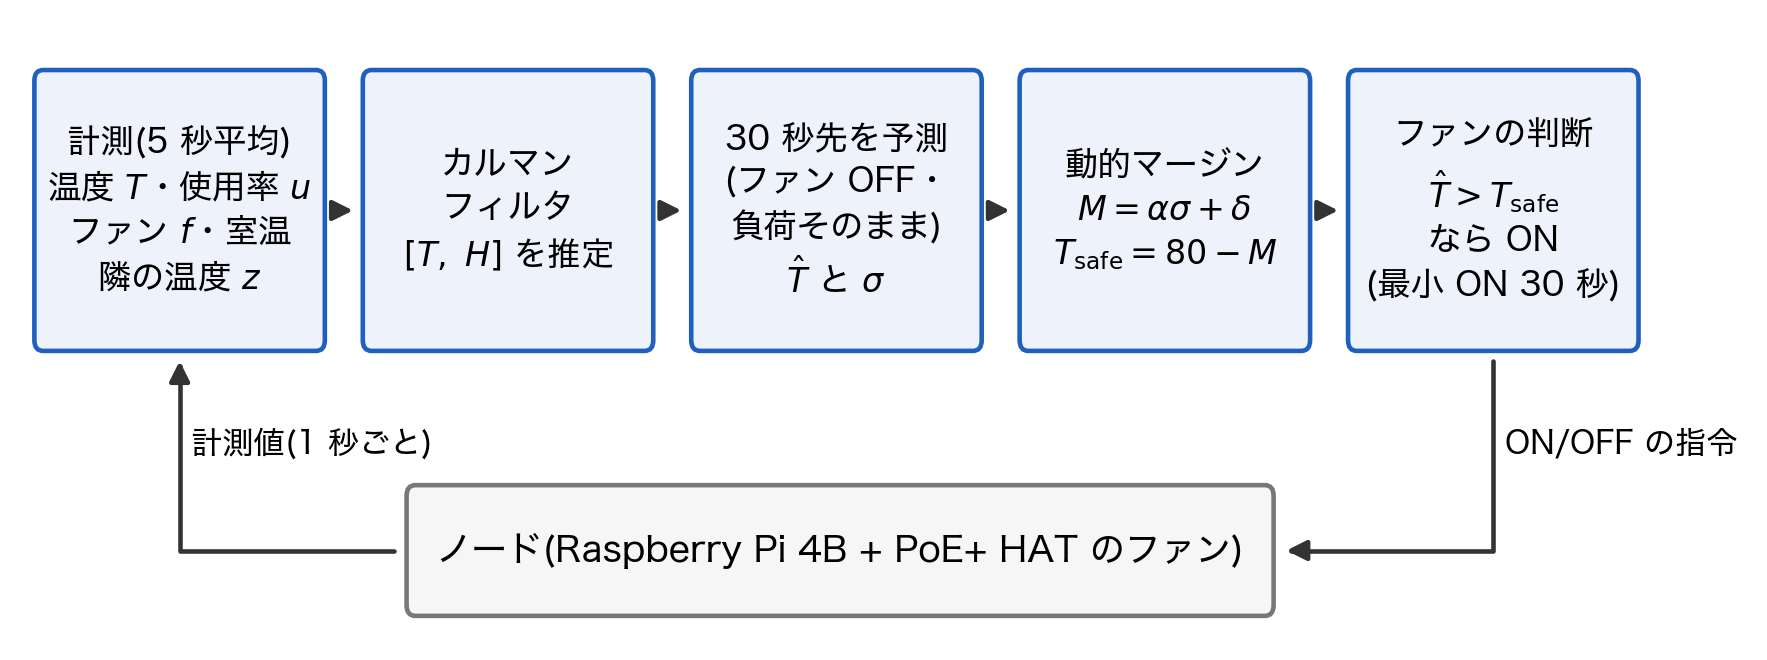
\includegraphics[width=0.85\textwidth]{fig_method_flow.png}
  \caption{提案手法の流れ(5 秒ごと)}
  \label{fig:flow}
\end{figure*}
手法の流れを図~\ref{fig:flow}に示す。5 秒ごとに、各ノードの温度・CPU 使用率・ファンの状態と、隣接ノードの温度を観測し、30 秒先の温度とその不確かさを予測して、ファンを回すかどうかを決める。

\subsection{外部熱影響を含む熱モデル}
1 台のノードを、熱をためる部分(熱容量)と逃がす部分(熱抵抗)からなる熱 RC モデルで表し、5 秒ごとに離散化する。温度は室温からの上昇分 $\theta_t = T_t - T_{\mathrm{amb}}$ で表す。
\begin{gather}
  \theta_{t+1} = a\,\theta_t + b\,u_t + c\,H_t + e\,f_t + d + w^{\theta}_t \label{eq:theta}\\
  H_{t+1} = \rho\,H_t + (1-\rho)\,z_t + w^{H}_t \label{eq:h}
\end{gather}
$u_t$ は CPU 使用率、$f_t$ はファンの状態(0/1)である。$a$ は熱の残り方(時定数 $\tau$ に対し $a = e^{-5/\tau}$)、$b > 0$ は負荷による加熱、$e < 0$ はファンによる冷却、$d$ は待機時の発熱を表す。

$H_t$ が外部熱影響である。$z_t$ は隣接ノードの温度の、普段の値からの変化分(隣接ノードの温度の平均から、アイドル時の平均を引いたもの)である。隣が熱くなると $z_t$ が大きくなり、$H_t$ はそれを $\rho$ でならしながら追いかける。その影響が係数 $c$ を通して自ノードの温度に現れる。隣が熱くなって自ノードが冷えることはないため、$c \ge 0$ とする。空間熱干渉が起こらない配置では、同定すると $c \approx 0$ となり、式~(\ref{eq:theta})は自ノードの負荷とファンだけのモデルに戻る。つまり、干渉の有無を前もって知らなくても、同じ手法を使える。

\subsection{カルマンフィルタによる推定と予測}
状態 $\bm{x}_t = [\theta_t, H_t]^\top$ のうち、観測できるのは $\theta_t$ だけである($y_t = \theta_t + v_t$)。カルマンフィルタで $\theta_t$ と $H_t$ を同時に推定する。隣接ノードの温度が急に変わったときは $H$ の変わり方も読みにくいため、$H$ のプロセスノイズを $q_H(t) = q_{H0} + \beta\,|z_t - z_{t-1}|$ と大きくする。

推定した状態から、式~(\ref{eq:theta})(\ref{eq:h})を 6 回(30 秒分)進めて、30 秒先の温度 $\hat{T}_{t+6|t}$ と、その誤差共分散 $P_{t+6|t}$ を求める。未来の負荷は分からないため今の負荷が続くと仮定し、ファンは OFF のままと仮定する。OFF と仮定するのは、「この先 30 秒回さなくても安全か」を判断するためである。30 秒は、ファンが効き始めるまでの時間(5 秒以内)より長く、温度の時定数(約 1〜2 分)より短い長さとして決めた。

\subsection{動的マージンとファン制御}
予測の不確かさ $\sigma_t = \sqrt{P_{t+6|t}[0,0]}$ からマージンを決める。
\begin{equation}
  M_t = \alpha\,\sigma_t + \delta,\qquad T_{\mathrm{safe}} = T_{\mathrm{limit}} - M_t
\end{equation}
$\alpha = 2$、$\delta = 0.5$\,℃(温度センサの刻み)、$T_{\mathrm{limit}} = 80$\,℃ とした。誤差が正規分布に従えば、予測 $+ 2\sigma$ を実測が超える確率は約 2.3\% である。隣の温度が急に変わると $q_H$ が大きくなり、$c > 0$ であれば $\sigma$ が広がってマージンが大きくなる。予測温度が $T_{\mathrm{safe}}$ を超えたらファンを ON にし、最小 ON 時間(30 秒)が過ぎて予測が $T_{\mathrm{safe}} - 1$\,℃ を下回ったら OFF にする。

\section{実験}
\subsection{何を確かめるか}
\begin{enumerate}
  \setlength{\itemsep}{0pt}\setlength{\parskip}{0pt}
  \item[Q1] 空間熱干渉は、どの位置関係(上・横・斜め・離れた位置)、どの発熱量、囲いの有無で起こるか
  \item[Q2] 冷やすときにも干渉は影響するか。(a) ファンの風で、排熱が隣に運ばれるか。(b) 隣が熱いと、自ノードのファンの冷え方が弱くなるか
  \item[Q3] 干渉が起こる条件で、$H$ を持つ予測は、持たない予測より当たるか
  \item[Q4] 予測に基づくファン制御は、スロットリングを避けつつファンの稼働を減らせるか
\end{enumerate}
Q1〜Q3 の条件と判定の基準は、測定の前に決めて記録した。

\subsection{実験環境}
\begin{figure}[tb]
  \centering
  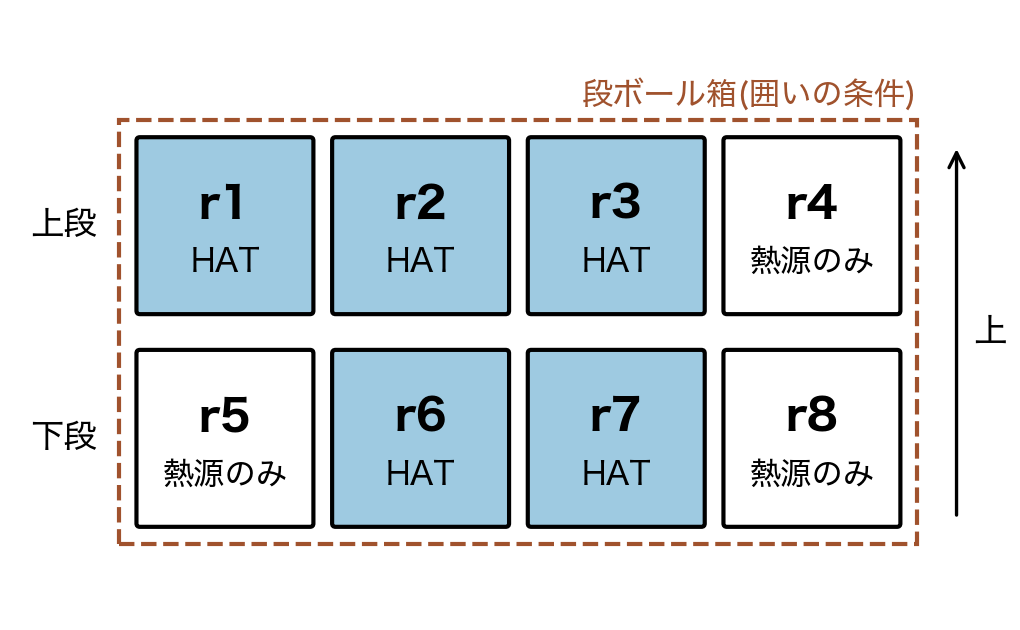
\includegraphics[width=\columnwidth]{fig_rack_layout.png}
  \caption{ラックの配置(ポート側から見た図)。網掛けは PoE+ HAT(ファン付き)のあるノード。囲いの条件では、ラック全体に段ボール箱をかぶせた}
  \label{fig:layout}
\end{figure}
Raspi 8 台(r1〜r8)を、2 段 × 4 列のラックに縦向きに固定した(図~\ref{fig:layout})。OS は Ubuntu 24.04 である。このうち 5 台(r1・r2・r3・r6・r7)には PoE+ HAT を付け、そのファンを制御用 PC から ON/OFF した。残りの 3 台は PoE+ HAT がなく(手元に 5 個しかなかったため)、ファンのない熱源として負荷だけを与えた。温度は 8 台すべてで記録した。1 秒ごとに温度・CPU 使用率・クロック・スロットリングの状態・ファンの状態を MQTT で集め、部屋の温度と、ラック(箱)の上部と正面の気温は温湿度計で記録した。負荷は \texttt{stress-ng} で与えた。

発熱量の目安として、PoE の給電電流(5\,V と仮定)から求めた 1 台の消費電力は、アイドルで約 2.4\,W、2 コアの負荷で約 3.8\,W、4 コアで約 5.3\,W であった\TBD{1 台だけ約 25\% 低く出る、要確認}。8 台に 2 コアの負荷をかけると、合わせて約 30\,W である。

\subsection{条件}
囲いは、なし(ラックがむき出し)と、段ボール箱(307 × 220 × 120\,mm、内容積約 8\,L)をラック全体にかぶせた状態の 2 通りとした。箱は上・左右・後ろを覆い、正面(ポート側)と下(ラックの脚の部分)は開いている。正面も閉じた箱では、アイドルだけで箱の上部の気温が 18 分で 39\,℃ まで上がり続けたため、決めていた 40\,℃ の手前で止めた。それぞれで次のブロックを順に行った(負荷は 2 コアで 10 分、その後 12 分休み)。
\begin{itemize}
  \setlength{\itemsep}{0pt}\setlength{\parskip}{0pt}
  \item 位置関係:下段の r6 だけ、r7 だけに負荷(ファンは全台 OFF)
  \item 発熱量:下段 4 台、8 台すべてに負荷
  \item Q2 (a):r6 のファンを ON にして r6 に負荷
  \item Q2 (b):r2 に負荷をかけ 10 分後に r2 のファンを ON。ほかの 7 台が休みのときと負荷中で冷え方を比べる
\end{itemize}
上昇は、負荷の最後 60 秒の平均温度から負荷の直前 60 秒の平均温度を引き、同じ間の室温の変化を引いた値とした。負荷をかけていないノードの上昇が 1\,℃ 以上なら「干渉あり」とする。

Q3 では、ファン OFF の区間で 30 秒先の予測を評価する。前半では上段に負荷がかからず負荷の係数が決まらないため、測定前の計画と逆に、後半で同定し前半(自ノードは休み、隣だけに負荷)で評価した。比べるのは、自ノードだけのモデル、$H$ を持つモデル(室温はどちらも部屋の温度)、自ノードだけで室温として上部(排気が当たる位置)または正面の気温を使うモデルの 4 つである。後の 2 つは、干渉が囲いの空気の昇温で説明できるかを見るために加えた。

Q4 は、横に 3 台並べた予備実験(11/14)で、0〜4 コアの負荷を切り替える 20 分のパターンを、ファンなし・常時 ON・しきい値方式(75\,℃ で ON、70\,℃ で OFF)・予測 + 固定マージン・提案手法の 5 条件で、順番をランダムにして 3 巡行った。

\section{結果}
\subsection{空間熱干渉が起こる条件(Q1)}
\begin{table}[tb]
  \centering
  \caption{負荷をかけていないノードの上昇(℃、室温の変化を引いた値)}
  \label{tab:pattern}
  \footnotesize\setlength{\tabcolsep}{2pt}
  \begin{tabular}{@{}lrr@{}}
    \toprule
    負荷 → 見るノード & 開いた状態 & 箱 \\
    \midrule
    真上(r6→r2、r7→r3) & $+0.1$, $+2.0$ & $-0.5$, $+0.5$ \\
    横(r6→r7、r7→r6) & $-1.4$, $+1.3$ & $-0.2$, $-0.2$ \\
    斜め上(r6→r1・r3, r7→r2) & $-0.3$, $-1.5$, $+1.0$ & $-0.1$, $-0.4$, $0.0$ \\
    離れた位置(r7→r1) & $+0.4$ & $+0.1$ \\
    \midrule
    下段 4 台 → 上段 r1〜r4 & $+0.6$〜$+1.4$ & $+0.1$〜$+1.8$ \\
    \bottomrule
  \end{tabular}
\end{table}
結果を表~\ref{tab:pattern}に示す(負荷をかけたノードは 10 分で 17〜21\,℃ 上がった)。開いた状態では、負荷をかけていないノードの上昇は、どの位置関係でも $-1.5$〜$+2.0$\,℃ の範囲であった。1\,℃ を超えたものもあるが、逆向き(r6 → r2、r6 → r7)はそろわず、r7 のブロックでは離れたノードも含めて全台が上がった。部屋の温度が 3 時間で 2.8\,℃ 変わっており、このブロックごとの揺れ(約 $\pm 1.5$\,℃)に、隣への干渉は埋もれる大きさであった。

一方、休みの間の温度は 3 時間で 4〜7\,℃ 上がり、8 台に同時に負荷をかけると 4 台が 80〜83\,℃ に達した(r6 だけのときは 77\,℃)。

箱では、負荷をかけていないノードの上昇は、どの位置関係でも $-0.5$〜$+0.5$\,℃ で、1\,℃ を超えたものはなかった。箱の中の気温はほぼ一定で、揺れは小さい。下段 4 台に負荷をかけると、上段の端の r1 が $+1.8$\,℃、r4 が $+1.3$\,℃ 上がったが、真上の r2・r3 は $+0.1$・$+0.2$\,℃ であった。

一方、囲うこと自体の影響は大きかった。負荷をかける前の温度は、部屋の温度の差(3.7\,℃)を引いても、開いた状態より 5〜10\,℃ 高く、上段ほど高かった。r6 だけに負荷をかけても 83.8\,℃ に達した(開いた状態では 77\,℃)。8 台に同時に負荷をかけると、ファン付きの 5 台がすべて 83\,℃ に達し、強制 ON が働いてクロックが下がった。

\subsection{冷やすときの干渉(Q2)}
\begin{figure}[tb]
  \centering
  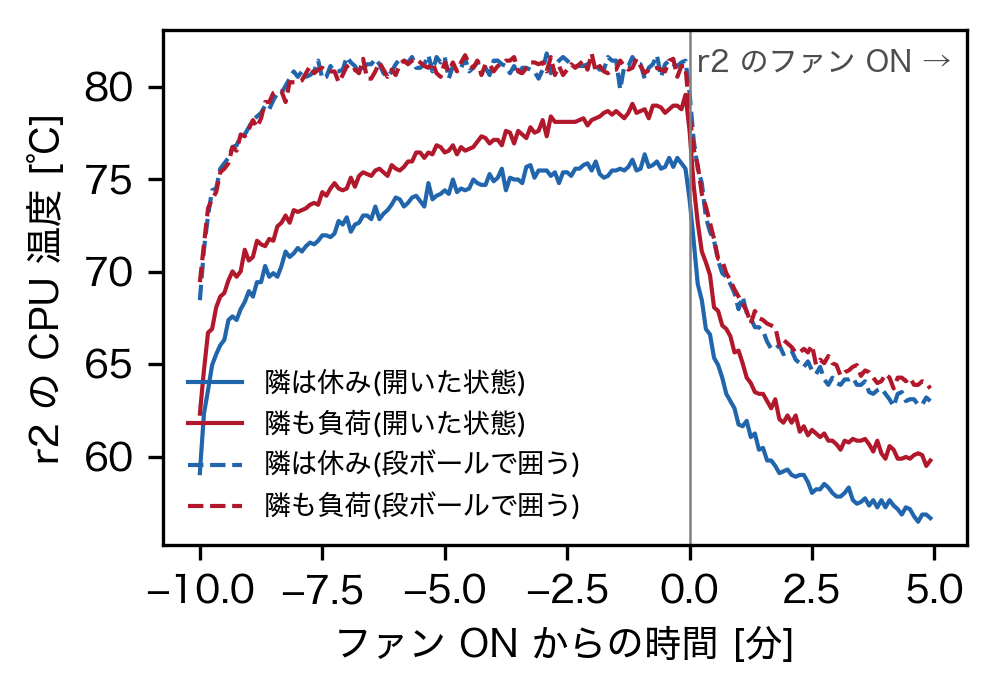
\includegraphics[width=0.72\columnwidth]{fig_pattern_cool.png}
  \caption{r2 のファンを ON にしたときの r2 の温度}
  \label{fig:cool}
\end{figure}
(a) r6 のファンを ON にしても、隣の上昇は OFF のときと比べて $\pm 1.4$\,℃ 以内(箱では $\pm 0.4$\,℃ 以内)で、開いた状態の揺れの範囲であった。

(b) 図~\ref{fig:cool}に示すように、ファンを ON にすると、ほかの 7 台が休みでも負荷中でも r2 は 18.8\,℃ 下がった。隣も負荷のときは ON の時点で 3\,℃ 高く、その差が残った。箱でも r2 は 17〜18\,℃ 下がり、5 分後の差は 1\,℃ 以内であった。

\subsection{予測の精度(Q3)}
\begin{table}[tb]
  \centering
  \caption{30 秒先の予測の平均絶対誤差(℃、上段 r1〜r3 の平均。評価は自ノードが休みで隣に負荷がかかる区間を含む前半)}
  \label{tab:pred}
  \small
  \begin{tabular}{lrr}
    \toprule
    モデル & 開いた状態 & 箱 \\
    \midrule
    自ノードのみ(室温 = 部屋) & 0.64 & 0.84 \\
    $H$ あり(室温 = 部屋) & \textbf{0.39} & 0.44 \\
    自ノードのみ(室温 = 上部の気温) & 0.69 & 0.53 \\
    自ノードのみ(室温 = 正面の気温) & 0.71 & \textbf{0.41} \\
    \bottomrule
  \end{tabular}
\end{table}
結果を表~\ref{tab:pred}に示す。開いた状態では、$H$ を持つモデルの誤差は自ノードだけのモデルより 0.25\,℃ 小さかった(基準とした 0.3\,℃ には届かない)。上部や正面の気温を使っても誤差は小さくならなかった。

箱では、$H$ を持つモデルの誤差は自ノードだけのモデルより 0.40\,℃ 小さく、基準の 0.3\,℃ を超えた。ただし、箱の正面の気温を室温として使った自ノードだけのモデルも 0.41\,℃ で、$H$ と同じ精度であった。r2 と r6 では $c < 0$ となり $H$ を外した。$\rho$ は多くのノードで 0.975〜0.995 であった。

\subsection{ファン制御(Q4)}
\begin{table}[tb]
  \centering
  \caption{ファン制御の結果(予備実験、9 回の平均。80\,℃ 超過は 20 分あたりの時間)}
  \label{tab:control}
  \small
  \begin{tabular}{lrrr}
    \toprule
    条件 & 稼働率 & 最高温度 & 80\,℃ 超過 \\
    \midrule
    ファンなし & 14\%$^{*}$ & 83.6\,℃ & 696 秒 \\
    常時 ON & 100\% & 65.0\,℃ & 0 \\
    しきい値 & 40\% & 78.4\,℃ & 0 \\
    予測 + 固定マージン & 45\% & 76.8\,℃ & 0 \\
    提案 & 38\% & 78.7\,℃ & 0 \\
    \bottomrule
    \multicolumn{4}{l}{\footnotesize $^{*}$ 82\,℃ 以上での安全のための強制 ON の分}
  \end{tabular}
\end{table}
結果を表~\ref{tab:control}に示す。予測を用いる 2 方式としきい値方式は、すべての回で 80\,℃ を超えず、スロットリングも起きなかった。提案手法は常時 ON と比べてファンの稼働を約 6 割減らした。$c \approx 0$ でも手法は壊れずに働いた。一方、しきい値方式との差はほぼなかった(38\% と 40\%)。

\section{考察}
\subsection{空間熱干渉が起こる条件}
本研究では、空間熱干渉を「ほかのノードの発熱によって自ノードの温度が上がること」とし、熱の経路は問わない。1 台の排気が隣を直接温める経路は、開いた状態でも箱でも、位置関係によらず 10 分の負荷では 1\,℃ 未満であった。一方、囲いやラックの空気に熱が溜まる経路は大きく、囲うだけで上段のアイドルの温度が 5〜10\,℃ 上がり、8 台に同時に負荷をかけると 80\,℃ を超えた。考慮が要るのは、隣に何があるかよりも、囲いの閉じ方と、同時に何台が動くかである。先行発表の約 12\,℃ の上昇も、密閉した小さな容器の中で溜まる経路が効いた結果と考えられる。

\subsection{外部熱影響 $H$ の役割}
箱では、箱の中の気温を室温として使うモデルが $H$ と同じくらい当たった。測定前に決めた解釈では、箱の中の干渉は主に箱全体の昇温であり、$H$ の役割は「箱の中に温度計がないときに、隣の温度からその昇温を推定する」ことである。開いた状態では、どの温湿度計を室温に使っても $H$ ほど当たらなかった。ラック全体の温まりは 1 か所の気温では捉えにくく、$H$ の方が適していた。

\subsection{しきい値方式と差がなかった理由}
PoE+ HAT のファンは 5 秒以内に効き始め効果も大きいため、温度が上がってから回しても間に合い、予測の利点が小さい。シミュレーションでは、効き始めが 15〜30 秒以上遅れると、予測を用いる方式が少ない稼働で 80\,℃ を守った。Q2 (b) では、隣が熱くてもファンの効きは弱まらず、干渉は温度の水準を押し上げるだけであった。予測が役立つのは、より遅い冷却の場合と考えられる。

\section{おわりに}
Raspi 8 台のラックで、位置関係・発熱量・囲い・ファンを変えて、空間熱干渉が起こる条件を実測した。1 台の排気が隣を直接温める干渉は 1\,℃ 未満で、熱は囲いやラックの空気に溜まる形で効いていた。$H$ は 30 秒先の予測誤差を 0.25〜0.40\,℃ 小さくし、箱の中の気温を使うのと同じ精度であった。今後は、囲いの大きさ・閉じ方と発熱量を変えて溜まる経路が効き始める条件を調べ、干渉が起こる配置でファン制御を評価する。

\scriptsize{
\begin{thebibliography}{99}
  \setlength{\itemsep}{0pt}
  \bibitem{moore} J. Moore et al., ``Making Scheduling ``Cool'': Temperature-Aware Workload Placement in Data Centers,'' USENIX ATC, pp.61--74, 2005.
  \bibitem{tang} Q. Tang et al., ``Energy-Efficient Thermal-Aware Task Scheduling for Homogeneous HPC Data Centers,'' IEEE TPDS, Vol.19, No.11, pp.1458--1472, 2008.
  \bibitem{iridis} S. J. Cox et al., ``Iridis-pi: a low-cost, compact demonstration cluster,'' Cluster Computing, pp.349--358, 2014.
  \bibitem{kim} S. J. Kim, A. Claassen, ``How to Evaluate Fan Life,'' Electronics Cooling, 1996.
  \bibitem{ipsj} 鈴木 黎映, 知念 賢一, ``空間熱干渉を考慮した状態推定に基づく動的熱マージン制御手法,'' 情報処理学会研究報告, Vol.2026-OS-171, No.3, 2026.
  \bibitem{zanini} F. Zanini et al., ``Multicore Thermal Management with Model Predictive Control,'' Proc. ECCTD, pp.711--714, 2009.
  \bibitem{sakamoto} 坂本 竜 他, ``仮想マシンの CPU 使用率の負荷予測に対する安定度を用いた動的マージン設定手法,'' 信学技報, Vol.117, No.465, pp.49--54, 2018.
  \bibitem{coskun} A. K. Coskun et al., ``Proactive Temperature Management in MPSoCs,'' Proc. ISLPED, 2008.
  \bibitem{yeo} I. Yeo et al., ``Predictive Dynamic Thermal Management for Multicore Systems,'' Proc. DAC, pp.734--739, 2008.
\end{thebibliography}
}
\end{document}
